\documentclass{beamer}

\mode<presentation>
{
	\usetheme{CambridgeUS}
	\setbeamercovered{transparent}
}

\setbeamertemplate{caption}[numbered]

\usepackage[spanish]{babel}
\usepackage[latin1]{inputenc}
\usepackage{color}
\usepackage{multicol}
\usepackage{listings}
\usepackage{hyperref}
\usepackage{algorithm,algorithmic}
\usepackage{colortbl}
\usepackage{graphicx}

\definecolor{mygreen}{rgb}{0,0.6,0}
\definecolor{mygray}{rgb}{0.5,0.5,0.5}
\definecolor{mymauve}{rgb}{0.58,0,0.82}

\lstset{ %
  backgroundcolor=\color{white},   % choose the background color; you must add \usepackage{color} or \usepackage{xcolor}
  basicstyle=\footnotesize,        % the size of the fonts that are used for the code
  breakatwhitespace=false,         % sets if automatic breaks should only happen at whitespace
  breaklines=true,                 % sets automatic line breaking
  captionpos=b,                    % sets the caption-position to bottom
  commentstyle=\color{gray},    % comment style
  deletekeywords={...},            % if you want to delete keywords from the given language
  escapeinside={\%*}{*)},          % if you want to add LaTeX within your code
  extendedchars=true,              % lets you use non-ASCII characters; for 8-bits encodings only, does not work with UTF-8
  frame=single,	                   % adds a frame around the code
  keepspaces=true,                 % keeps spaces in text, useful for keeping indentation of code (possibly needs columns=flexible)
  keywordstyle=\color{blue},       % keyword style
  language=Octave,                 % the language of the code
  otherkeywords={else},           % if you want to add more keywords to the set
  numbers=left,                    % where to put the line-numbers; possible values are (none, left, right)
  numbersep=5pt,                   % how far the line-numbers are from the code
  numberstyle=\tiny\color{mygray}, % the style that is used for the line-numbers
  rulecolor=\color{black},         % if not set, the frame-color may be changed on line-breaks within not-black text (e.g. comments (green here))
  showspaces=false,                % show spaces everywhere adding particular underscores; it overrides 'showstringspaces'
  showstringspaces=false,          % underline spaces within strings only
  showtabs=false,                  % show tabs within strings adding particular underscores
  stepnumber=2,                    % the step between two line-numbers. If it's 1, each line will be numbered
  stringstyle=\color{mymauve},     % string literal style
  tabsize=2,	                   % sets default tabsize to 2 spaces
  title=\lstname                   % show the filename of files included with \lstinputlisting; also try caption instead of title
}

\title[\textbf{Programaci\'on 2}]{\textbf{Programaci\'on 2}}

\subtitle{Java Database Connectivity (\emph{JDBC})}

\author[Rodrigo Olivares]
{
	Rodrigo Olivares \\
	\vspace{0.5mm}
	Mg. en Ingenier\'ia Inform\'atica \\
	\vspace{0.5mm}
	\texttt{\normalsize rodrigo.olivares@uv.cl}
}

\institute[Universidad de Valpara\'iso]

\date{$1^{er}$ Semestre de 2016} 

\subject{Programaci\'on 2}


\AtBeginSection
{
	\begin{frame}<beamer>
	\frametitle{Contenido}
	\tableofcontents[currentsection,currentsubsection]
	\end{frame}
}

\AtBeginSubsection
{
	\begin{frame}<beamer>
	\frametitle{Contenido}
	\tableofcontents[currentsection,currentsubsection]
	\end{frame}
}

\beamerdefaultoverlayspecification{<+->}

\begin{document}

	\begin{frame}
		\titlepage
	\end{frame}

	\begin{frame}
		\frametitle{Contenido}
		\tableofcontents[pausesections]
	\end{frame}

    \section{JDBC}

    \subsection{Introducci\'on}

	\begin{frame}
		\frametitle{JDBC}
		\framesubtitle{Introducci\'on}

		\begin{block}{Introducci\'on}
		    \begin{itemize}
		        \item Aplicaci\'on que procese informaci\'on \textbf{base de datos}.
		        \item Normalmente se utilizan bases de datos relacionales.
		        \item SQL: Lenguaje est\'andar para acceder a una base datos.
		    \end{itemize}
		\end{block}
	\end{frame}
	
    \subsection{Caracter\'isticas de JDBC}	
	
	\begin{frame}
		\frametitle{JDBC}
		\framesubtitle{Caracter\'isticas de JDBC}

		\begin{block}{Caracter\'isticas de JDBC }
		    \begin{itemize}
		        \item Es un interfaz orientado a objetos de Java para SQL.
		        \item Se utiliza para enviar sentencias SQL a un sistema gestor de BD (DBMS).
		        \item Con JDBC tenemos que continuar escribiendo las sentencias SQL.
		    \end{itemize}
		\end{block}
	\end{frame}

	\begin{frame}
		\frametitle{JDBC}
		\framesubtitle{Caracter\'isticas de JDBC}

		\begin{block}{Caracter\'isticas de JDBC }
		    \begin{itemize}
		        \item La filosof\'ia de JDBC es proporcionar transparencia al desarrollador frente al gestor de BD.
		        \item JDBC utiliza un Gestor de Controladores o \textbf{DriverManager} que hace de interfaz con el controlador espec\'ifico de la BD.
		    \end{itemize}
		\end{block}
	\end{frame}

	\begin{frame}
		\frametitle{JDBC}
		\framesubtitle{Caracter\'isticas de JDBC}

		    \begin{center}
				\fbox{\fbox{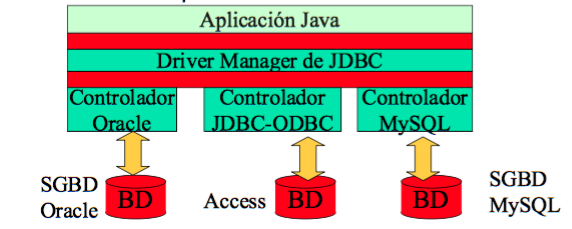
\includegraphics[scale=.55]{images/arquitectura-jdbc.png}}}
			\end{center}
	\end{frame}

	\begin{frame}
		\frametitle{JDBC}
		\framesubtitle{Caracter\'isticas de JDBC}

		\begin{block}{Caracter\'isticas de JDBC }
		    \begin{itemize}
		        \item La especificaci\'on JDBC incluye 8 interfaces y 10 clases, en el paquete est\'andar \textbf{java.sql}.
		        \item Podemos dividirlos en los siguientes grupos: N\'ucleo de JDBC, interfaces y clases que todos los controladores deben implementar.
		        \begin{itemize}
		            \item Extensiones al paquete \textbf{java.lang}, extensiones para SQL.
		            \item Extensiones al paquete \textbf{java.util}, son extensiones a \textbf{java.util.Date}.
		            \item Metadatos para SQL, permiten examinar din\'amicamente las propiedades de BD y controladores.
		        \end{itemize}
		    \end{itemize}
		\end{block}
	\end{frame}

	\begin{frame}
		\frametitle{JDBC}
		\framesubtitle{Caracter\'isticas de JDBC}

		    \begin{center}
				\fbox{\fbox{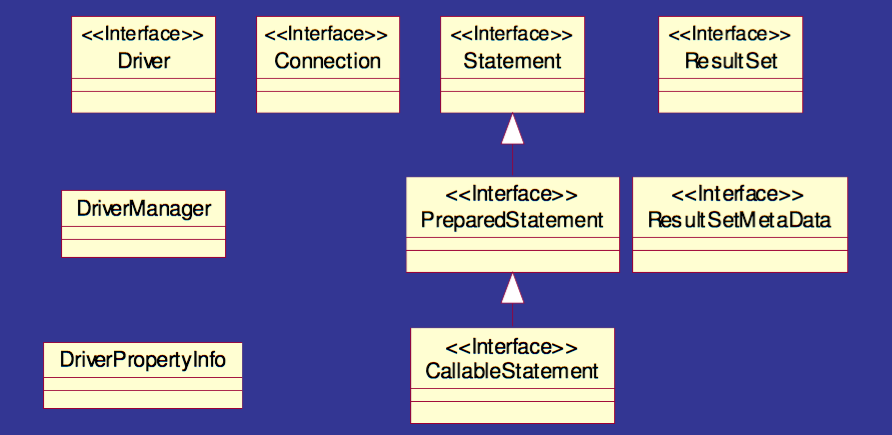
\includegraphics[scale=.35]{images/nucleo-jdbc.png}}}
			\end{center}
	\end{frame}

    \subsection{Pasos para una conexi\'on JDBC}	

	\begin{frame}
		\frametitle{JDBC}
		\framesubtitle{Pasos para una conexi\'on JDBC - Primer paso}

        \begin{exampleblock}{Pasos para una conexi\'on JDBC - Primer paso}
		    \begin{itemize}
		        \item Antes de conectar con la base de datos, debemos considerar dos aspectos:
		        \begin{itemize}
		            \item Registrar un controlador.
		            \item Convenciones de nombres para la base de datos.
		        \end{itemize}
		    \end{itemize}
		    \end{exampleblock}
	\end{frame}

	\begin{frame}
		\frametitle{JDBC}
		\framesubtitle{Pasos para una conexi\'on JDBC - Primer paso}

        \begin{exampleblock}{Registrar un controlador}
		    \begin{itemize}
		        \item Determinados controladores requerir\'an la instalaci\'on y configuraci\'on de software espec\'ifico en el cliente. Ejemplo: el origen ODBC o la fuente de datos nativa.		        
		        \item Otros controladores son simplemente una clase Java y bastar\'a que la \textbf{Java Virtual Machine} las pueda localizar mediante el \textbf{classpath}.
		    \end{itemize}
		    \end{exampleblock}
	\end{frame}

    \begin{frame}
		\frametitle{JDBC}
		\framesubtitle{Pasos para una conexi\'on JDBC - Primer paso}

        \begin{exampleblock}{Registrar un controlador}
		    \begin{itemize}
		        \item Para que la JVM pueda localizar una clase de driver, se debe:
		        \begin{itemize}
		            \item \underline{Situar la ruta a la clase en el \emph{CLASSPATH}}.
		            \item \textbf{A\~nadir un JAR externo en el proyecto donde est\'a nuestra aplicaci\'on.}
		            \item Configurar una asociaci\'on o pool de conexiones (ambientes web).
		        \end{itemize}
		    \end{itemize}
		\end{exampleblock}
	\end{frame}	
	
	\begin{frame}
		\frametitle{JDBC}
		\framesubtitle{Pasos para una conexi\'on JDBC - Primer paso}

        \begin{exampleblock}{Registrar un controlador}
		    \begin{itemize}
		        \item Averiguar el nombre de la clase provista por el paquete a ser usado.
		        \item Localizar la clase en el directorio apropiado para que pueda ser cargado.
		        \item Alternativamente se puede cargar la clase en el programa usando el comando:
		        \begin{itemize}
		            \item \textbf{Class.forName(``sun.jdbcJdbcOdbcDriver")}
		            \item \textbf{DriverManager.registerDriver(new oracle.jdbc.driver.OracleDriver())}.
		        \end{itemize}
		    \end{itemize}
		\end{exampleblock}
	\end{frame}	
	
	\begin{frame}
		\frametitle{JDBC}
		\framesubtitle{Pasos para una conexi\'on JDBC - Primer paso}

        \lstinputlisting[language=Java,caption={},numbers=none]{resources/code1.java}       
	\end{frame}		
	
	\begin{frame}
		\frametitle{JDBC}
		\framesubtitle{Pasos para una conexi\'on JDBC - Segundo paso}

        \begin{exampleblock}{Pasos para una conexi\'on JDBC - Segundo paso}
		    \begin{itemize}
		        \item La clase \textbf{DriverManager} es la responsable de:
		        \begin{itemize}
		            \item Seleccionar el driver.
		            \item Crear una nueva conexi\'on a la base de datos.
		        \end{itemize}
		        \item Previamente habremos registrado el controlador en el \textbf{DriverManager}.
		    \end{itemize}
		    \end{exampleblock}
	\end{frame}
	
	\begin{frame}
		\frametitle{JDBC}
		\framesubtitle{Pasos para una conexi\'on JDBC - Segundo paso}

        \begin{exampleblock}{Pasos para una conexi\'on JDBC - Segundo paso}
		    \begin{itemize}
		        \item Crear una conexi\'on:
		        \begin{itemize}
		            \item \textbf{Connection con = DriverManager.getConnection(url,user,pass)}
		        \end{itemize}
		        \item El par\'ametro imprescindible es la url de la base de datos; para especificar la base de datos que queremos utilizar.
		        \item Tambi\'en se puede especificar el usuario y la clave con los que nos queremos conectar a la base de datos.
		        \item El \textbf{DriverManager} buscar\'a un driver, entre los registrados que pueda usar el protocolo especificado en la url.
		    \end{itemize}
		    \end{exampleblock}
	\end{frame}	
	
	\begin{frame}
		\frametitle{JDBC}
		\framesubtitle{Pasos para una conexi\'on JDBC - Segundo paso}

        \begin{exampleblock}{Pasos para una conexi\'on JDBC - Segundo paso}
		    \begin{itemize}
		        \item En JDBC las bases de datos se designan mediante una URL.
		        \item La forma de la url es la siguiente: \textbf{jdbc:<subprotocolo>:<dominio>}
		        \item \textbf{Subprotocolo}: identifica el mecanismo de conexi\'on o el controlador JDBC concreto.
		        \item \textbf{Dominio}: Depende del subprotocolo, puede ser simplemente un nombre simple para la base de datos o una serie de par\'ametros que permiten encontrar la BD.
		    \end{itemize}
		    \end{exampleblock}
	\end{frame}
  
	\begin{frame}
		\frametitle{JDBC}
		\framesubtitle{Pasos para una conexi\'on JDBC - Segundo paso}

        \begin{exampleblock}{Pasos para una conexi\'on JDBC - Segundo paso}
		    \begin{itemize}
		        \item Si no se producen excepciones el m\'etodo \textbf{getConnection} nos devuelve un objeto que implementa la interfaz \textbf{Connection}.
		        \item Podemos crear varias conexiones con distintas bases de datos o incluso con la misma.
		        \item Cada conexi\'on representa una sesi\'on con la BD.
		        \item El objeto \textbf{Connection} nos permitir\'a acceder a la base de datos para realizar operaciones sobre ella y obtener resultados.
		    \end{itemize}
		    \end{exampleblock}
	\end{frame}  
  
	\begin{frame}
		\frametitle{JDBC}
		\framesubtitle{Pasos para una conexi\'on JDBC - Segundo paso}

        \lstinputlisting[language=Java,caption={},numbers=none]{resources/code2.java}       
	\end{frame}

	\begin{frame}
		\frametitle{JDBC}
		\framesubtitle{Pasos para una conexi\'on JDBC - Tercer paso}

        \begin{exampleblock}{Pasos para una conexi\'on JDBC - Tercer paso}
		    \begin{itemize}
		        \item Utilizamos la conexi\'on con la base de datos creada anteriormente para enviar comandos y sentencias SQL.
		        \item El objeto conexi\'on funciona como un enlace directo con el controlador de la BD.
		        \item Creamos un objeto de la clase \textbf{Statement} que servir\'a de \emph{envoltorio} para las sentencias SQL.
		        \item Cuando pasamos la SQL a la conexi\'on este lo env\'ia al controlador que a su vez lo redirecciona a la BD, que nos devolver\'a los resultados.
		    \end{itemize}
		    \end{exampleblock}
	\end{frame}    
 
	\begin{frame}
		\frametitle{JDBC}
		\framesubtitle{Pasos para una conexi\'on JDBC - Tercer paso}

        \begin{exampleblock}{Pasos para una conexi\'on JDBC - Tercer paso}
		    \begin{itemize}
		        \item La clase \textbf{Connection} tiene varios m\'etodos que permiten crear un objeto \textbf{Statement} o una de sus variantes.
		        \item \textbf{createStatement}, para crear sentencias simples.
		        \item prepareStatement, para sentencias que pueden contener par\'ametros, optimiza la utilizaci\'on repetida de estas sentencias.
		        \item prepareCall, para funciones o procedimientos almancenados.
		    \end{itemize}
		    \end{exampleblock}
	\end{frame}    	
	
    \begin{frame}
		\frametitle{JDBC}
		\framesubtitle{Pasos para una conexi\'on JDBC - Tercer paso}

        \lstinputlisting[language=Java,caption={},numbers=none]{resources/code3.java}       
	\end{frame}		
	
	\begin{frame}
		\frametitle{JDBC}
		\framesubtitle{Pasos para una conexi\'on JDBC - Cuarto paso}

        \begin{exampleblock}{Pasos para una conexi\'on JDBC - Cuarto paso}
		    \begin{itemize}
		        \item Ejecuci\'on
		        \begin{itemize}
		            \item \textbf{executeQuery}(), ejecuci\'on de consultas, sentencia SELECT.
		            \item \textbf{executeUpdate}(), actualizaciones de valores en al base de datos. I\textbf{NSERT, UPDATE, DELETE}. S\'olo devuelve la cuenta de las columnas afectadas.
		            \item \textbf{execute}(), se usa para ejecutar sentencias que no se conocen a priori o que devuelven resultados no homog\'eneos.
		        \end{itemize}
		    \end{itemize}
		    \end{exampleblock}
	\end{frame}    		
	
    \begin{frame}
		\frametitle{JDBC}
		\framesubtitle{Pasos para una conexi\'on JDBC - Cuarto paso}

        \lstinputlisting[language=Java,caption={},numbers=none]{resources/code4.java}       
	\end{frame}			
	
	\begin{frame}
		\frametitle{JDBC}
		\framesubtitle{Pasos para una conexi\'on JDBC - Quinto paso}

        \begin{exampleblock}{Pasos para una conexi\'on JDBC - Quinto paso}
		    \begin{itemize}
		        \item Recuperaci\'on
		        \begin{itemize}
		            \item Cuando ejecutamos una consulta debemos emplear el m\'etodo \textbf{executeQuery}(), que devuelve un objeto \textbf{ResultSet}, que nos permitir\'a acceder a los resultados.
		            \item El \textbf{ResultSet} utiliza el concepto de cursor de base de datos para ir movi\'endose por las filas de datos recuperadas.
		            \item Las columnas pueden accederse en cualquier orden, utilizando su posici\'on o su nombre.
		            \item El objeto \textbf{ResultSet} incluye m\'etodos getXXX que permiten recuperar valores de distintos tipos.
		        \end{itemize}
		    \end{itemize}
		    \end{exampleblock}
	\end{frame}   	
	
    \begin{frame}
		\frametitle{JDBC}
		\framesubtitle{Pasos para una conexi\'on JDBC - Quinto paso}

        \lstinputlisting[language=Java,caption={},numbers=none]{resources/code5.java}       
	\end{frame}			
	
    \begin{frame}
		\frametitle{Preguntas}

		\hspace{4cm}\huge{Preguntas ?}
		
	\end{frame}
	
\end{document}

\usetheme{default}
\usetheme{JuanLesPins}
\usetheme{Goettingen}
\usetheme{Szeged}
\usetheme{Warsaw}

\usecolortheme{crane}

\usefonttheme{serif}
\usefonttheme{structuresmallcapsserif}
